\section{LOS DATOS}\label{sec:los-datos}

\subsection{Tipos de Variables}\label{sec:tiposdevariables}

Dentro de las 47 variables descriptivas a utilizar antes mencionadas también se incluyen 4 variables que muestran la evolución temporal por intervalos de los pacientes. Estas variables son:

\begin{itemize}
    \item Flujo de Oxígeno
    \item Frecuencia Respiratoria (FR)
    \item Escala SAPI (Sistemas de Alerta Precoz Infantil)
    \item Score Wood-Downes
\end{itemize}

Estas 4 variables no han sido tratadas como series temporales dada la baja frecuencia de recolección durante las primeras 24 h de ingreso; que es el intervalo temporal al que ha sido acotado el estudio. Las tres primeras (Flujo de Oxígeno, Frecuencia Respiratoria y Escala SAPI)variables han sido recopiladas 3 veces durante las primeras 24h del ingreso del paciente pediátrico y la última (Score Wood-Downes) ha sido recogida a la llegada del paciente y a las 24 h. Es decir estas variables describen la estancia del paciente en intervalos.  Estas variables serán catalogadas como \textit{Temporales en Intervalos.} 

Si tratamos estas 3 últimas variables como temporales nos quedarían solamente 36 variables descriptivas. (3 variables temporales $\times$ 3 intervalos + 1 $\times$ 2 intervalos = 11 variables) y por otro lado 2 variables en forma de series temporales. Cada variable de estas contiene 1441 datos. (60 minutos $\times$ 24 horas + 1\textsuperscript{er} dato repetido
= 1441).

Dentro de las 36 variables descriptivas restantes se encuentran 3 variables que dan información más allá de las primeras 24 h de monitorización. Estas variables en principio serán excluidas del estudio y son:

\begin{itemize}
    \item Días con Gafas Nasales
    \item Días con O$_2$
    \item Días con OAF
\end{itemize}

Estas 3 variables serán catalogadas como: \textit{Descriptivas fuera del scope}. El \textit{scope} será básicamente las primeras 24 h de ingreso del paciente pediátrico.

Por último dentro de las 33 variables descriptivas dentro del \textit{scope} se encuentran 2 variables que no son ni cualitativas ni cuantitativas. Estas variables serán catalogadas como \textit{Otras}. Las 31 variables restantes serán catalogadas como \textit{Descriptivas dentro de scope}.

En la tabla \ref{tabla:variables_estudio} se muestran las diferentes variables recopiladas para realizar el presente estudio. 

\begin{table}[H]
    \centering
        \begin{tabular}{| m{5cm} | m{1.75cm} | m{7cm} |}
            \hline Tipo de Variable & Cantidad & Nombres  \\ \hline
            Descriptivas dentro de scope & 31 & Edad, Peso, Sexo, Edad Gestacional (EG), Palivizumab, Lactancia Materna (LM), Dermatitis, Alergias, Tabaco, Enfermedad Base, Radiografía, Analítica, Suero, Etiología, Prematuridad, Alimentación, Sonda Nasogástrica, Gafas Nasales al Ingreso, OAF, OAF al ingreso, OAF tras ingreso, Horas de Ingreso tras inicio OAF, UCIP, Deterioro, Pausas de Apnea, PCT (Procalcitonina en la sangre), PCR (Prueba de Proteína C relativa), Leucocitos, Nautrófilos, Linfocitos y Score Cruces Ingreso  \\ \hline
            Descriptivas fuera de scope & 3 & Días con Gafas Nasales, Días con O$_2$ y Días con OAF. \\ \hline
            Temporales en 3 Intervalos & 11 & Frecuencia Respiratoria (0 - 8 h), Frecuencia Respiratoria (8 - 16 h),
            Frecuencia Respiratoria (16 - 24 h),
            Flujo O$_2$ (0 - 8 h),
            Flujo O$_2$ (8 - 16 h),
            Flujo O$_2$ (16 - 24 h),
            SAPI (0 - 8 h),
            SAPI (8 - 16 h), 
            SAPI (16 - 24 h), Score Wood-Downes Ingreso y Score Wood-Downes 24 h . \\ \hline
            Series Temporales & 2 & Frecuencia Cardiaca, Saturación de Oxígeno \\ \hline
            Otras & 2 & Notas e Identificador Paciente. \\ \hline
        \end{tabular}
    \caption{Variables Usadas en el Estudio}\label{tabla:variables_estudio}
\end{table}

Las variables temporales han sido recopiladas durante las primeras 24 h del ingreso del paciente pediátrico cuando mostraba un cuadro bronquiolítico. La frecuencia con la que han sido recopilados los datos ha sido de 1 vez cada minuto. En la siguiente Figura \ref{fig:fc-JJB} se muestra un ejemplo de la evolución  variable \textit{Frecuencia Cardiaca} en forma de serie temporal y de la misma forma la Figura \ref{fig:satO2-JJB} pero para la \textit{Saturación de O$_2$}. Estas dos series temorales pertenecen a la evolución del paciente pediátrico \textit{JJB\_11182744}.

\begin{figure}[H]
    \centering
    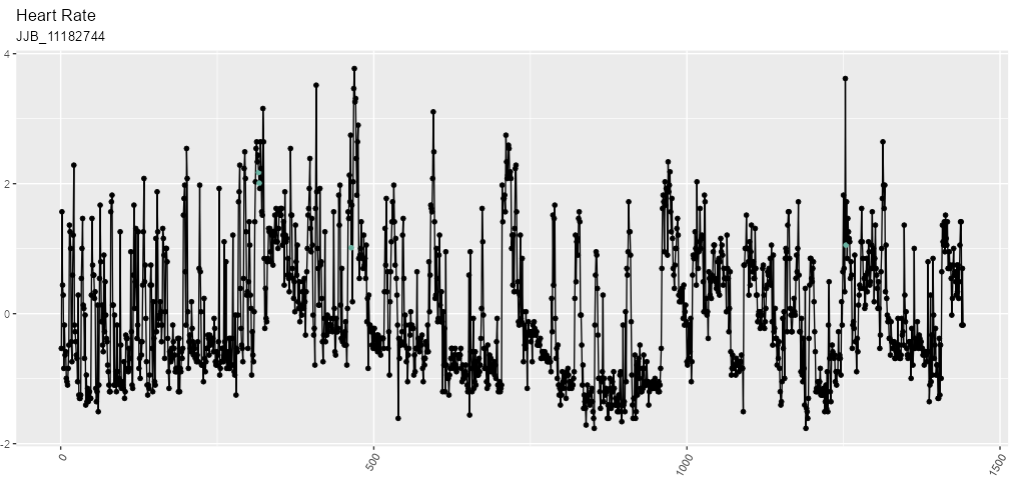
\includegraphics[scale=0.70]{./img/Heart-Rate-JJB.png}
    \caption{Valores de Frecuencia Cardíaca del paciente \textit{JJB\_11182744}}
    \label{fig:fc-JJB}
\end{figure}

\begin{figure}[H]
    \centering
    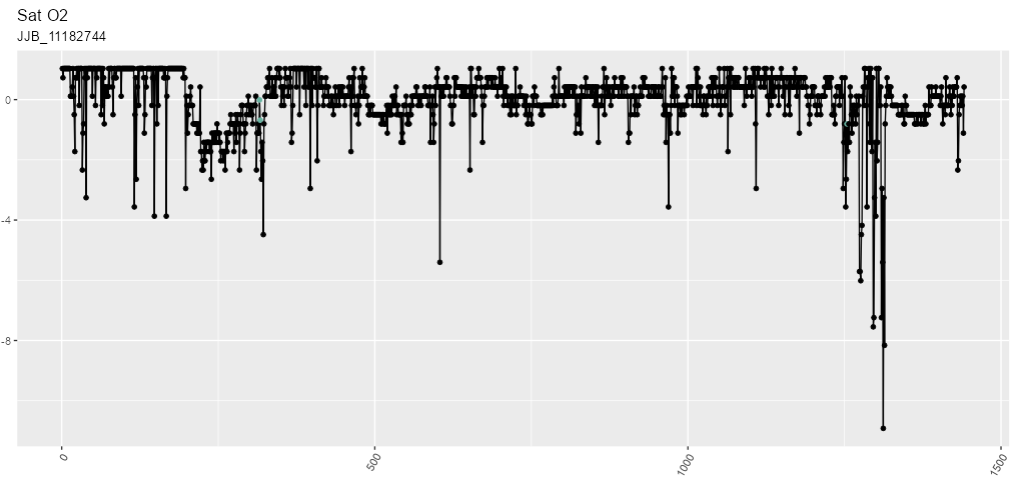
\includegraphics[scale=0.70]{./img/SatO2-JJB.png}
    \caption{Valores de Saturación de O$_2$ del paciente \textit{JJB\_11182744}}
    \label{fig:satO2-JJB}
\end{figure}

A la hora de trabajar con variables temporales se ha de tener en cuenta que los datos temporales pueden ser de dos tipos: \textit{Discretos} o \textit{Continuos}. Los datos discretos son aquellos que se recogen en intervalos de tiempo, por ejemplo, el número de pacientes que llegan a un hospital cada hora. Los datos continuos son aquellos que se recogen de forma continua, por ejemplo, en nuestro caso la saturación y frecuencia cardíaca de un paciente cada minuto.

Para terminar esta Sección \ref{sec:tiposdevariables} una última cuestión a valorar son las variables cualitativas y cuantitativas que se han recopilado. Las variables cualitativas son aquellas que describen una cualidad del paciente, por ejemplo, el sexo o la edad gestacional. Las variables cuantitativas son aquellas que describen una cantidad del paciente, por ejemplo, la frecuencia cardíaca o la saturación de oxígeno.

En la siguiente Tabla \ref{tabla:cuali_cuanti} se muestra la división entre variables cualitativas y cuantitivas recopiladas en el estudio y dentro del \textit{scope}.

\begin{table}[H]
    \centering
        \begin{tabular}{| m{5cm} | m{1.75cm} | m{7cm} |}
            \hline Tipo de Variable & Cantidad & Nombres  \\ \hline
            Cuantitativas & 15 & Edad, Peso, Edad Gestacional (EG), Horas de Ingreso tras inicio OAF, PCT (Procalcitonina en la sangre), PCR (Prueba de Proteína C relativa), Leucocitos, Nautrófilos, Linfocitos, Frecuencia Respiratoria (0 - 8 h), Frecuencia Respiratoria (8 - 16 h),
            Frecuencia Respiratoria (16 - 24 h),
            Flujo O$_2$ (0 - 8 h),
            Flujo O$_2$ (8 - 16 h),
            Flujo O$_2$ (16 - 24 h). \\ \hline
            Cualitativas & 27 & Sexo, Palivizumab, Lactancia Materna (LM), Dermatitis, Alergias, Tabaco, Enfermedad Base, Radiografía, Analítica, Suero, Etiología, Prematuridad, Alimentación, Sonda Nasogástrica, Gafas Nasales al Ingreso, OAF, OAF al ingreso, OAF tras ingreso, UCIP, Deterioro, Pausas de Apnea, Score Cruces Ingreso, SAPI (0 - 8 h),
            SAPI (8 - 16 h), 
            SAPI (16 - 24 h), Score Wood-Downes Ingreso y Score Wood-Downes 24 h. \\ \hline
            Otras & 2 & Notas e Identificador Paciente. \\ \hline
        \end{tabular}
    \caption{Variables Cualitativas y Cuantitativas Dentro del \textit{Scope}}\label{tabla:cuali_cuanti}
\end{table}

\subsection{Preprocesamiento de los Datos}

En este apartado se describirá el procesamiento de los datos realizado para el presente estudio.

\subsubsection{Limpieza de Datos}

En primer lugar se ha realizado una limpieza de datos. Esta limpieza de datos ha consistido en varios pasos: 

\begin{enumerate}
    \item \textbf{Validación de Archivos:} Contrastar que los diferentes archivos de datos no contienen datos duplicados o incoherencias.
    \item \textbf{Cálculo de Medias:} Calcular de manera automatizada las medias de \textit{Frecuencia Respiratoria} y \textit{Saturación de Oxígeno} cada hora. Estas medias han sido facilitadas en el Archivo de Datos de Pacientes pero por rigor se han vuelto a calcular para cada paciente. Ya que además que en la Carpeta de Datos de Monitorización se guardan los datos brutos con los que los médicos han calculado estas medias. Además de estas $2$ medias horarias, se han hecho dos trasformaciones en los datos de \textit{Frecuencia Cardiaca} que se explicarán más tarde. (\textit{Frecuencia Cardiaca Escalada} y \textit{Frecuencia Cardiaca por Cuantiles})
    \item \textbf{Datos Faltantes:} Determinar que pacientes y variables tienen un alto número de datos faltantes y eliminarlos del estudio.
    \item \textbf{Variables No Relevantes:} Eliminar variables que no aportan información relevante para el estudio.
\end{enumerate}

 \paragraph*{Validación de Archivos}

Por parte del hospital se han recopilado 2 archivos de datos diferentes. Estos archivos de datos son:

\begin{itemize}
    \item \textbf{Archivo de Datos de Pacientes:} Este archivo contiene información descriptiva de los pacientes pediátricos. En este archivo se encuentran las variables contenidas en la Tabla \ref{tabla:cuali_cuanti}. Este archivo contiene 47 variables y 79 pacientes.
    \item \textbf{Carpeta de Datos de Monitorización:} En esta carpeta se almacena un archivo por cada paciente. Cada archivo contiene información temporal de los pacientes pediátricos. En este archivo se encuentran las variables \textit{Series Temporales} en la Tabla \ref{tabla:variables_estudio}. Por cada archivo se tienen 2 variables temporales (Saturación de O$_2$ y Frecuencia Cardiaca), cada variable presenta 1441 datos por paciente.
\end{itemize}

La Carpeta de Datos de Monitorización contiene 79 archivos de datos y el Archivo de Datos de Pacientes contiene 79 pacientes. Por lo tanto, se ha de contrastar que los datos de los pacientes contenidos en el Archivo de Datos de Pacientes estén contenidos en la Carpeta de Datos de Monitorización o si existen pacientes duplicados.

La cabecera de la Carpeta de Datos de Monitorización es la siguiente:
\begin{figure}[H]
    \centering
    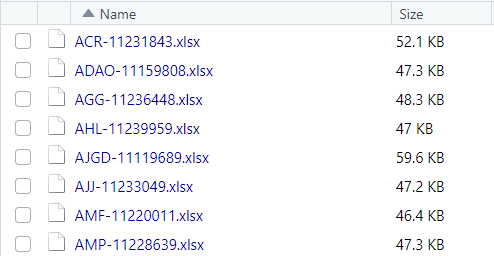
\includegraphics[scale=0.70]{./img/Carpeta-Monitor.png}
    \caption{Cabecera de la Carpeta de Datos de Monitorización}
    \label{fig:cabecera_monitorizacion}
\end{figure}

Y las primeras columnas del Archivo de Datos de Pacientes son las siguientes:
\begin{figure}[H]
    \centering
    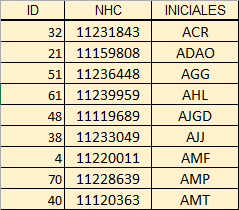
\includegraphics[scale=1.0]{./img/Archivo-Monitor.png}
    \caption{Cabecera de la Carpeta de Datos de Monitorización}
    \label{fig:cabecera_monitorizacion}
\end{figure}

Este contraste se ha automatizado de manera que para futuros estudios se pueda realizar de manera rápida y eficiente. El resultado de este contraste ha sido que los datos de los pacientes contenidos en el Archivo de Datos de Pacientes están contenidos en la Carpeta de Datos de Monitorización. Existían algunas desviaciones en los nombres pero fuero corregidas. Por lo tanto, no existen pacientes duplicados y se puede continuar con el estudio.

\paragraph*{Cálculo de Medias}

En el Archivo de Datos de Pacientes venían calculadas las medias de \textit{Frecuencia Respiratoria} y \textit{Flujo de Oxígeno} cada hora. Estas medias han sido re-calculadas de manera automatizada para cada paciente y se han añadido al Archivo de Datos de Pacientes. Además de estas 2 medias se han hecho dos trasformaciones en los datos de \textit{Frecuencia Cardiaca} que se explicarán más tarde y se han calculado sus respectivas medias por hora. 

Se han calculado dos tipos de medias: 

\begin{itemize}
    \item \textbf{Medias No Nulas:} Se han calculado las medias de aquellos intervalos de hora dentro de las 24 h que no presentaban valores faltantes.
    \item \textbf{Medias Nulas:} Se han calculado las medias de aquellos intervalos de hora dentro de las 24 h sin importar si había momentos de valores valores faltantes dentro del intervalo hora.
\end{itemize}

Estos valores se han calculado para todos los pacientes, como modo de ejemplo el resultado para el paciente \textit{JJB\_11182744} ha sido el siguiente mostrado en la Tabla \ref{tabla:medias-JJB}:

% Se comienza una página nueva sin formato (sin número de página y sin encabezado/pie de página):
\newpage
\thispagestyle{empty}

% Se modifica la geometría (los márgenes) de la página y se coloca en formato horizontal:
\newgeometry{top=10mm, bottom=10mm, left=12mm, right=12mm}
\begin{landscape}

    \begin{table}[!ht]
        \centering
        \begin{tabular}{|l|l|l|l|l|l|l|l|l|l|l|l|}
        \hline
            hour & n & Missing\_FC & Missing\_SO2 & Mean\_FC & Mean\_SO2 & Mean\_Q & Mean\_SC & Mean\_FC\_NA & Mean\_SO2\_NA & Mean\_Q\_NA & Mean\_SC\_NA \\ \hline
            18 & 43 & 0 & 0 & 140,4186047 & 98,23255814 & 0,552067823 & -0,205230874 & 140,4186047 & 98,23255814 & 0,552067823 & -0,205230874 \\ \hline
            19 & 60 & 0 & 0 & 137,4666667 & 99,1 & 0,500688619 & -0,356544211 & 137,4666667 & 99,1 & 0,500688619 & -0,356544211 \\ \hline
            20 & 60 & 0 & 0 & 143,0166667 & 98,46666667 & 0,613802318 & -0,07205686 & 143,0166667 & 98,46666667 & 0,613802318 & -0,07205686 \\ \hline
            21 & 60 & 0 & 0 & 141,7 & 97,13333333 & 0,567600299 & -0,139547853 & 141,7 & 97,13333333 & 0,567600299 & -0,139547853 \\ \hline
            22 & 60 & 0 & 0 & 135,3666667 & 92,11666667 & 0,479248047 & -0,464188074 & 135,3666667 & 92,11666667 & 0,479248047 & -0,464188074 \\ \hline
            23 & 60 & 2 & 2 & ~ & ~ & ~ & ~ & 164,3448276 & 95,12068966 & 0,867006799 & 1,021202963 \\ \hline
            00 & 60 & 0 & 0 & 162,0666667 & 98,5 & 0,918496135 & 0,904426753 & 162,0666667 & 98,5 & 0,918496135 & 0,904426753 \\ \hline
            01 & 60 & 0 & 0 & 150,9833333 & 97,13333333 & 0,729509118 & 0,336306366 & 150,9833333 & 97,13333333 & 0,729509118 & 0,336306366 \\ \hline
            02 & 60 & 1 & 0 & ~ & 95,98333333 & ~ & ~ & 155,559322 & 95,98333333 & 0,762103523 & 0,570866889 \\ \hline
            03 & 60 & 0 & 0 & 142,3166667 & 96,01666667 & 0,606131522 & -0,107938147 & 142,3166667 & 96,01666667 & 0,606131522 & -0,107938147 \\ \hline
            04 & 60 & 0 & 0 & 142,2166667 & 96,86666667 & 0,569912026 & -0,113064045 & 142,2166667 & 96,86666667 & 0,569912026 & -0,113064045 \\ \hline
            05 & 60 & 0 & 0 & 130,6166667 & 97,8 & 0,37096502 & -0,70766824 & 130,6166667 & 97,8 & 0,37096502 & -0,70766824 \\ \hline
            06 & 60 & 0 & 0 & 155,8166667 & 96,4 & 0,762258703 & 0,584058113 & 155,8166667 & 96,4 & 0,762258703 & 0,584058113 \\ \hline
            07 & 60 & 0 & 0 & 132,55 & 96,73333333 & 0,405018753 & -0,608567541 & 132,55 & 96,73333333 & 0,405018753 & -0,608567541 \\ \hline
            08 & 60 & 0 & 0 & 129,4833333 & 97,06666667 & 0,344631214 & -0,765761753 & 129,4833333 & 97,06666667 & 0,344631214 & -0,765761753 \\ \hline
            09 & 60 & 0 & 0 & 127,8166667 & 97,18333333 & 0,312055141 & -0,85119339 & 127,8166667 & 97,18333333 & 0,312055141 & -0,85119339 \\ \hline
            10 & 60 & 0 & 0 & 151,2166667 & 96,43333333 & 0,703296936 & 0,348266795 & 151,2166667 & 96,43333333 & 0,703296936 & 0,348266795 \\ \hline
            11 & 60 & 0 & 0 & 156,55 & 97,41666667 & 0,87619425 & 0,621648034 & 156,55 & 97,41666667 & 0,87619425 & 0,621648034 \\ \hline
            12 & 60 & 0 & 0 & 145,95 & 98,1 & 0,685284072 & 0,078302822 & 145,95 & 98,1 & 0,685284072 & 0,078302822 \\ \hline
            13 & 60 & 0 & 0 & 146,4166667 & 98,13333333 & 0,704465169 & 0,10222368 & 146,4166667 & 98,13333333 & 0,704465169 & 0,10222368 \\ \hline
            14 & 60 & 0 & 0 & 129,9333333 & 97,08333333 & 0,372386073 & -0,742695211 & 129,9333333 & 97,08333333 & 0,372386073 & -0,742695211 \\ \hline
            15 & 60 & 1 & 1 & ~ & ~ & ~ & ~ & 155,220339 & 92,6779661 & 0,833584194 & 0,553490963 \\ \hline
            16 & 60 & 0 & 0 & 143,6333333 & 93,95 & 0,628285376 & -0,040447154 & 143,6333333 & 93,95 & 0,628285376 & -0,040447154 \\ \hline
            17 & 60 & 0 & 0 & 141,8666667 & 96,01666667 & 0,596238571 & -0,131004689 & 141,8666667 & 96,01666667 & 0,596238571 & -0,131004689 \\ \hline
            18\_1 & 18 & 0 & 0 & 156,1111111 & 96,05555556 & 0,890367072 & 0,599151036 & 156,1111111 & 96,05555556 & 0,890367072 & 0,599151036 \\ \hline
        \end{tabular}
        \caption{Medias Nulas y No Nulas de \textit{Frecuencia Cardíaca}, \textit{Saturación de O$_2$}, \textit{Cuantiles Cardíacos} y \textit{Frecuencia Cardíaca Escalada}  por hora para el paciente \textit{JJB\_11182744}}\label{tabla:medias-JJB}
    \end{table}

% Se devuelve el formato y la geometría de la página a sus valores originales:
\end{landscape}
\restoregeometry 

\paragraph*{Datos Faltantes}

Se ha realizado un estudio de los datos faltantes. Este estudio ha consistido en determinar que pacientes y que variables tenían un alto número de datos faltantes y eliminarlos del estudio. 

\subparagraph*{Variables con Datos Faltantes} 

En la siguiente Imagen \ref{fig:missing-descriptive} se muestra la distribución de datos faltantes de las variables referenciadas en la Tabla \ref{tabla:cuali_cuanti}. 
 
\begin{figure}[H]
    \centering
    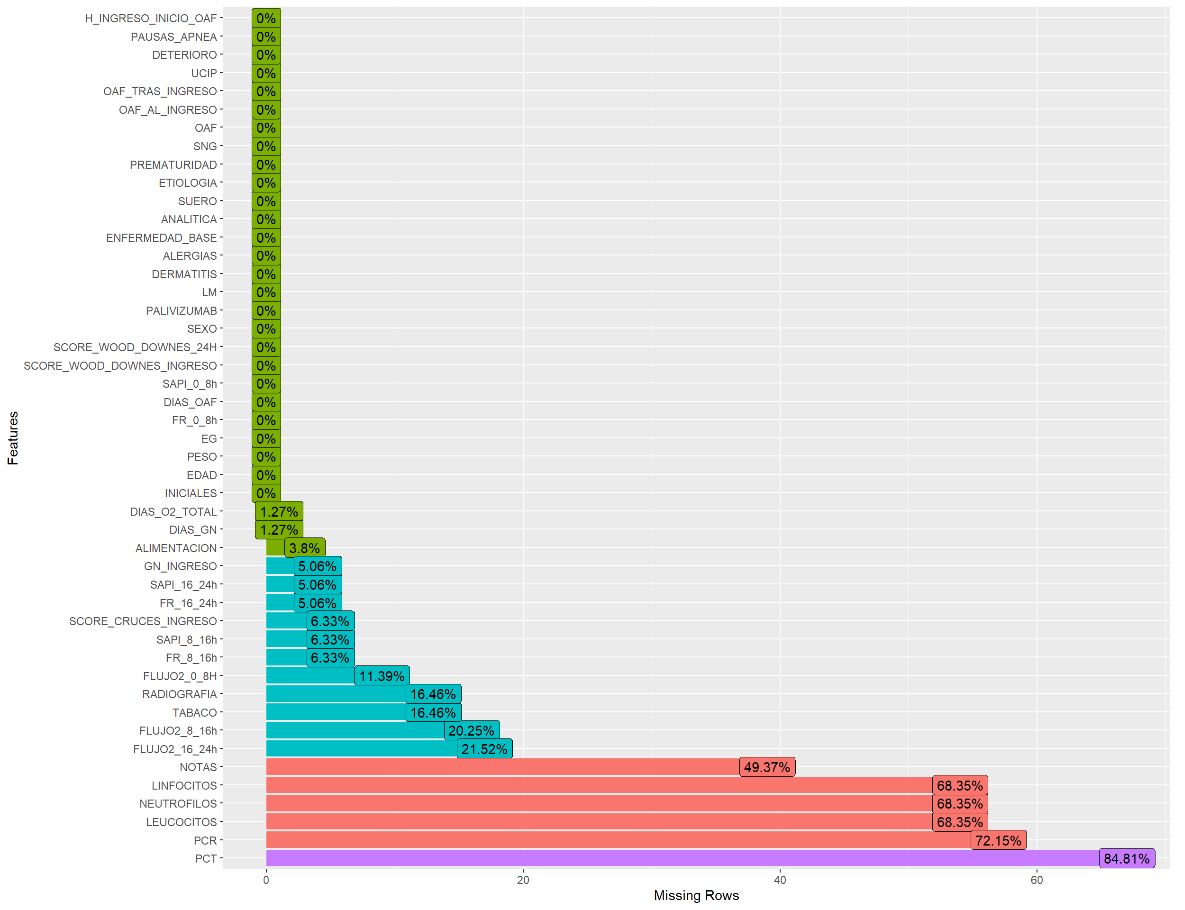
\includegraphics[scale = 0.70]{./img/missig-data-descriptive.png}
    \caption{Datos Faltantes en el Archivo de Datos de Pacientes}
    \label{fig:missing-descriptive}
\end{figure}

Por tro lado se ha estudiado que variables suelen faltar juntas. En la siguiente Imagen \ref{fig:missing-descriptive-cross} se muestra la distribución de datos faltantes cruzados de las 6 variables con mayor número de datos faltantes de la anterior Figura \ref{fig:missing-descriptive}.

\begin{figure}[H]
    \centering
    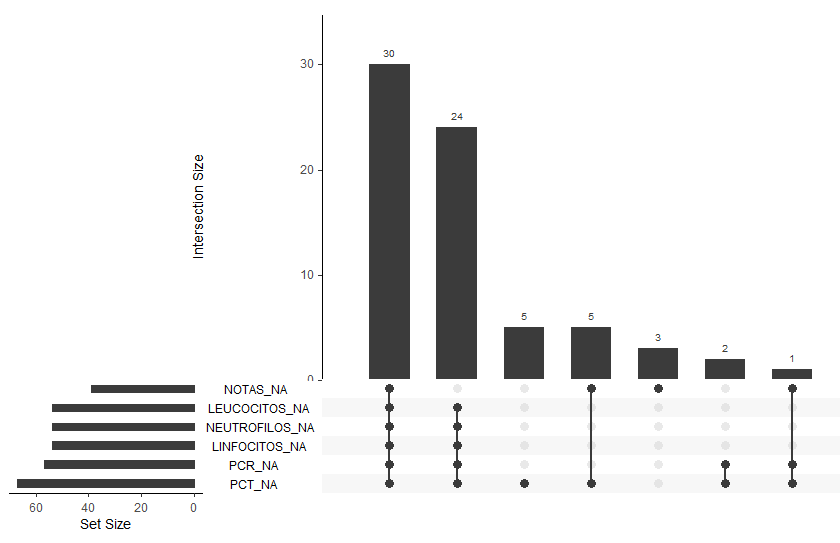
\includegraphics[scale = 0.70]{./img/missig-data-descriptive-cross.png}
    \caption{Datos Faltantes Cruzados de las 6 variables con Mayor Porcentaje de Datos Faltantes en el Archivo de Datos de Pacientes}
    \label{fig:missing-descriptive-cross}
\end{figure}

Según la Figura \ref{fig:missing-descriptive-cross} los \textit{Neutrofilos}, \textit{Linfocitos} y \textit{Leucocitos} se muestran faltantes siempre juntos, si falta uno faltan todos. Esto tiene sentido ya que los tres se obtienen si al paciente se le ha realizado una analítica. Por el contrario si solo contamos con los pacientes a los que se les ha realizado una analítica no hay faltantes de estas tres variables como se puede ver en la Figura \ref{fig:missing-descriptive-cross-analitica}. Es decir de manera sencilla, los datos faltantes de estas tres variables se deben a que no se le ha realizado una analítica al paciente.

\begin{figure}[H]
    \centering
    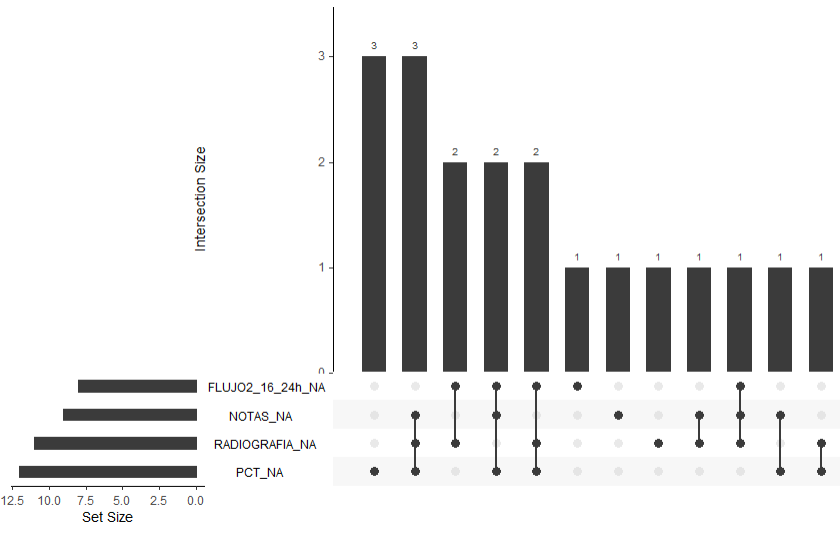
\includegraphics[scale = 0.70]{./img/missig-data-descriptive-cross-anal.png}
    \caption{Datos Faltantes Cruzados de las 4 variables con Mayor Porcentaje de Datos Faltantes en el Archivo de Datos de Pacientes si se le Ha Realizado una Analítica al Paciente}
    \label{fig:missing-descriptive-cross-analitica}
\end{figure}
\newpage




\subparagraph*{Pacientes con Datos Faltantes} 

Cuando se habla de pacientes con datos faltantes se hace referencia a aquellos pacientes que tienen datos faltantes en las variables \textit{Series Temporales} de la Tabla \ref{tabla:variables_estudio}. 

A cada paciente se le monitoriza durante las primeras 24 horas de su ingreso. En algunos casos, pueden ocurrir eventos que interrumpan la monitorización continua. Por ejemplo, si un paciente es trasladado a la Unidad de Cuidados Intensivos Pediátricos (UCIP), si es necesario realizarle alguna prueba o llevar a cabo tareas de higiene personal, se le desconecta de la monitorización. 

En la Figuras \ref{fig:fc-HGSDA} y \ref{fig:satO2-HGSDA} se muestran las \textit{Series Temporales} de \textit{Frecuencia Cardiaca} y \textit{Saturación de O$_2$} de el paciente \textit{HGSDA\_11233118} respectivamente. En estas se pueden observar como en ciertos momentos la monitorización se pausa y se registran valores faltantes en ciertos intervalos. 
\begin{figure}[H]
    \centering
    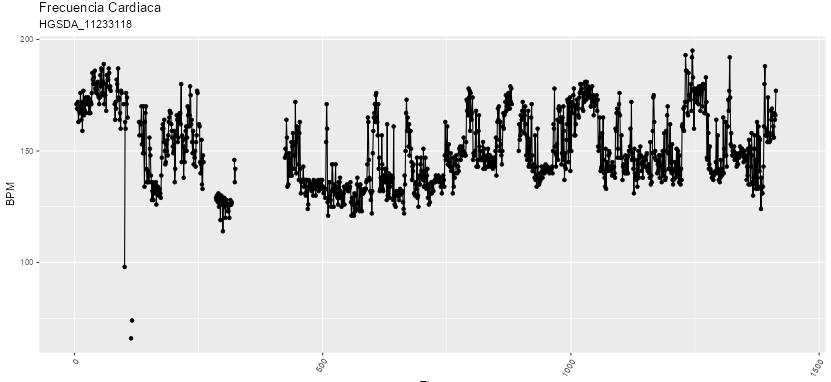
\includegraphics[scale=0.85]{./img/Heart-Rate-HGSDA.png}
    \caption{Valores de Frecuencia Cardíaca del paciente \textit{HGSDA\_11233118}}
    \label{fig:fc-HGSDA}
\end{figure}

\begin{figure}[H]
    \centering
    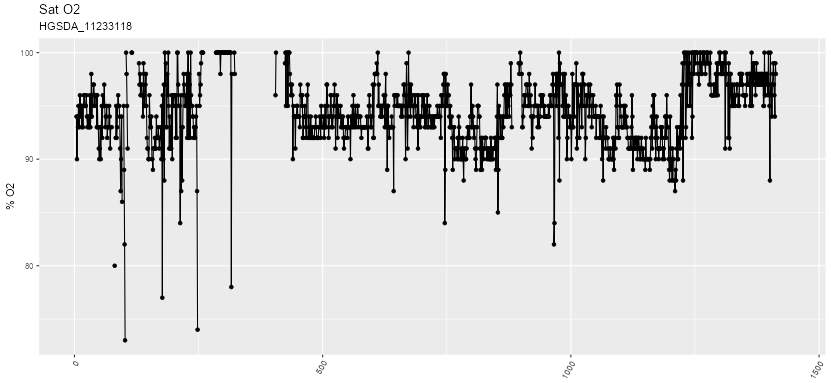
\includegraphics[scale=0.85]{./img/SatO2-HGSDA.png}
    \caption{Valores de Saturación de O$_2$ del paciente \textit{HGSDA\_11233118}}
    \label{fig:satO2-HGSDA}
\end{figure}


En la siguientes Figuras \ref{fig:missing-FC} y \ref{fig:missing-SatO2} se muestra la distribución y porcentaje de datos faltantes en las \textit{Series Temporales} de los 79 pacientes estudiados. La primera imagen hace referencia a la \textit{Frecuencia Cardiaca} y la segunda a la \textit{Saturación de O$_2$}.

% Se comienza una página nueva sin formato (sin número de página y sin encabezado/pie de página):
\newpage
\thispagestyle{empty}

% Se modifica la geometría (los márgenes) de la página y se coloca en formato horizontal:
\newgeometry{top=10mm, bottom=10mm, left=12mm, right=12mm}
\begin{landscape}

    \begin{figure}[H]
        \centering
        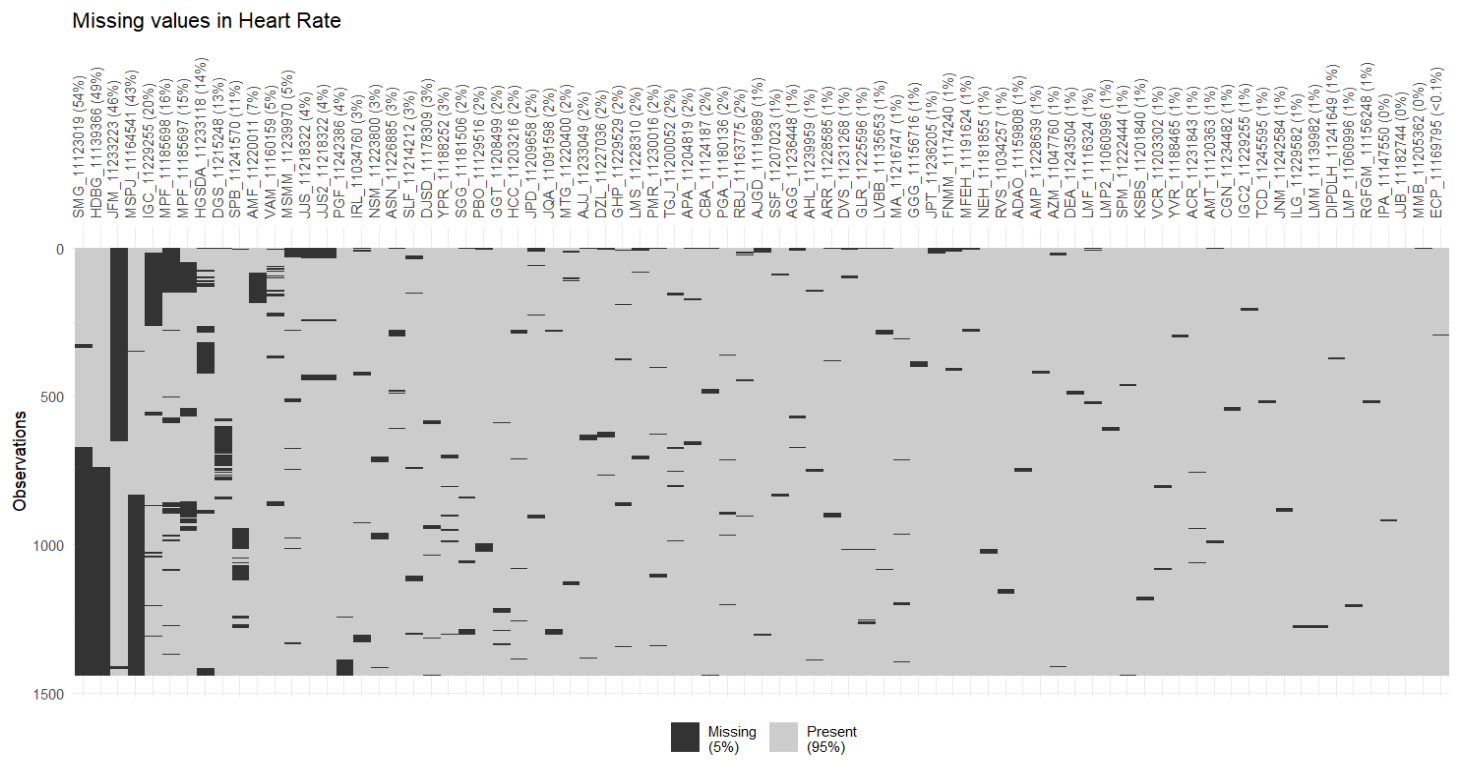
\includegraphics[scale = 0.9]{./img/missing-data-HR.png}
        \caption{Datos Faltantes en la \textit{Frecuencia Cardiaca} de los 79 pacientes pediátricos}
        \label{fig:missing-FC}
    \end{figure}
    
% Se devuelve el formato y la geometría de la página a sus valores originales:
\end{landscape}
\restoregeometry 

\newpage
\thispagestyle{empty}

% Se modifica la geometría (los márgenes) de la página y se coloca en formato horizontal:
\newgeometry{top=10mm, bottom=10mm, left=12mm, right=12mm}
\begin{landscape}

    \begin{figure}[H]
        \centering
        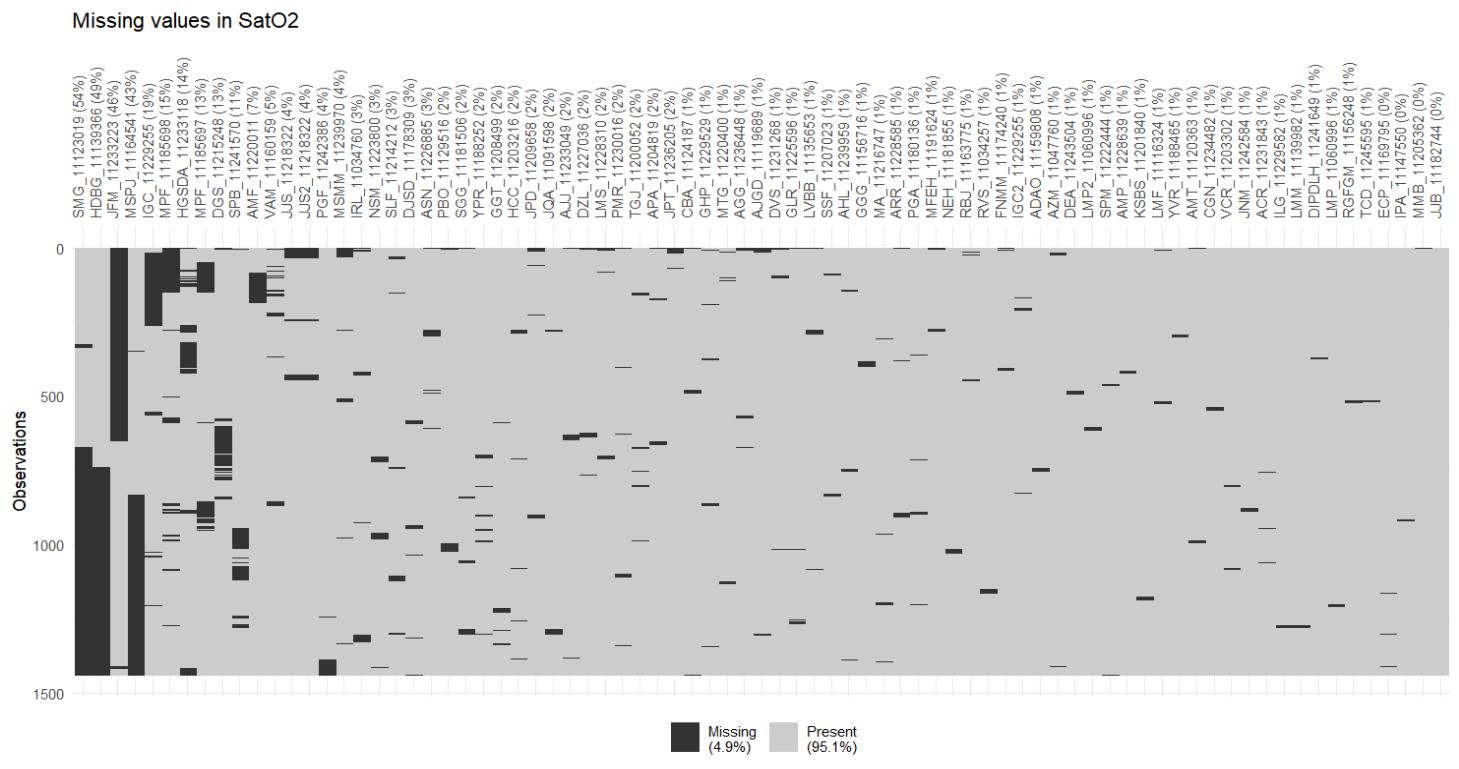
\includegraphics[scale = 0.9]{./img/missing-data-SatO2.png}
        \caption{Datos Faltantes en la \textit{Saturación de O$_2$} de los 79 pacientes pediátricos}
        \label{fig:missing-SatO2}
    \end{figure}
    
% Se devuelve el formato y la geometría de la página a sus valores originales:
\end{landscape}
\restoregeometry 

 A la hora de determinar los pacientes que van a ser incluidos en el estudio se va a tener en cuenta la variable \textit{Deterioro}. Esta variable indica si el paciente ha sufrido un deterioro durante las primeras 24 h de ingreso. Se considera \textit{Deterioro} si el paciente ha sido trasladado a la UCIP o ha recibido Oxigenación de Alto Flujo. 

 Estudiando los datos se ve como todos los pacientes que han sido trasladados a la UCIP han tenido previamente una intervención en la que se les ha aplicado Oxigenación de Alto Flujo pero no a todos a los que se les ha aplicado Oxigenación de Alto Flujo han sido trasladados a la UCIP. De esta forma los pacientes que muestren \textit{Deterioro} serán los mismos a los que se les ha aplicado OAF. Esto se puede ver en el diagrama de Venn en la Figura \ref{fig:venn-OAF-UCIP}.

\begin{figure}[H]
    \centering
    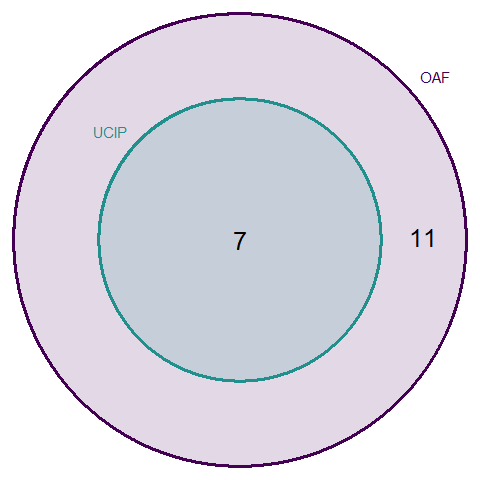
\includegraphics[scale = 0.75]{./img/venn-diagram-OAF-UCIP.png}
    \caption{Diagrama de Venn de los pacientes que han sido trasladados a la UCIP 7 y los que han recibido OAF $12 + 7 = 19$}
    \label{fig:venn-OAF-UCIP}
\end{figure}


Se utilizará la variable \textit{Deterioro} como indicadora de que el paciente ha sufrido un deterioro durante las primeras 24 h de ingreso. A la hora de eliminar pacientes será interesante ver cómo afecta también a la proporción de pacientes que han sufrido un deterioro y los que no. En la siguiente Tabla \ref{tabla:ratio-deterioro} se muestra la cantidad de pacientes que presentan \textit{Deterioro}, los que no y el ratio entre \textit{Deterioro} y no \textit{Deterioro}.


\begin{table}[H]
    \centering
    \begin{tabular}{|m{2cm}|m{2.25cm}|m{2cm}|m{2cm}|}
    \hline
        Pacientes Totales & No Deterioro & Deterioro & Ratio \\ \hline
        79 & 61 & 18 & 0.295082 \\ \hline
    \end{tabular}
    \caption{Pacientes Totales, con Deterioro, sin Deterioro y Ratio entre Deterioro y No Deterioro}
        \label{tabla:ratio-deterioro}
\end{table}

\newpage

Se van a plantear dos metodologías para establecer la exclusión de pacientes en el estudio en función de las variables \textit{Series Temporales} de \textit{Frecuencia Cardiaca} y \textit{Saturación de O$_2$}. El objetivo es ver cómo varían la cantidad de pacientes incluidos en el estudio en ambos casos: 

\begin{itemize}
    \item \textbf{Método 1:} Se va a establecer un \textit{threshold} en el $5 \%$ de valores faltantes . Una vez establecido dicho \textit{threshold} se va a ir aumentando el tiempo de \textit{scope} del estudio. Es decir en vez de plantear estudiar las 24 primeras horas se va a estudiar si centrándose en un intervalo menor de estudio existen más pacientes que cumplen este criterio de admisión. Se va a ir aumentando el intervalo de estudio desde las 8 primeras h en intervalos de 30 minutos hasta las primeras 15 horas. Es decir se va a estudiar si existen más pacientes que cumplen el criterio de admisión en las primeras 8 horas, en las primeras $8.5$ horas, en las primeras $7$ horas, etc. hasta llegar a las 15 horas. Este método se puede ver en la Figura \ref{fig:metodo1}.
    \item \textbf{Método 2:} Se va a ir aumentando el \textit{threshold} desde el $5 \%$ hasta el $20 \%$ en intervalos de $2.5 \%$.  Es decir se va a estudiar si existen más pacientes que cumplen el criterio de admisión en las primeras $24$ horas cambiando el \textit{threshold}. Este método se puede ver en la Figura \ref{fig:metodo2}.
\end{itemize}

\begin{figure}[H]
    \centering
    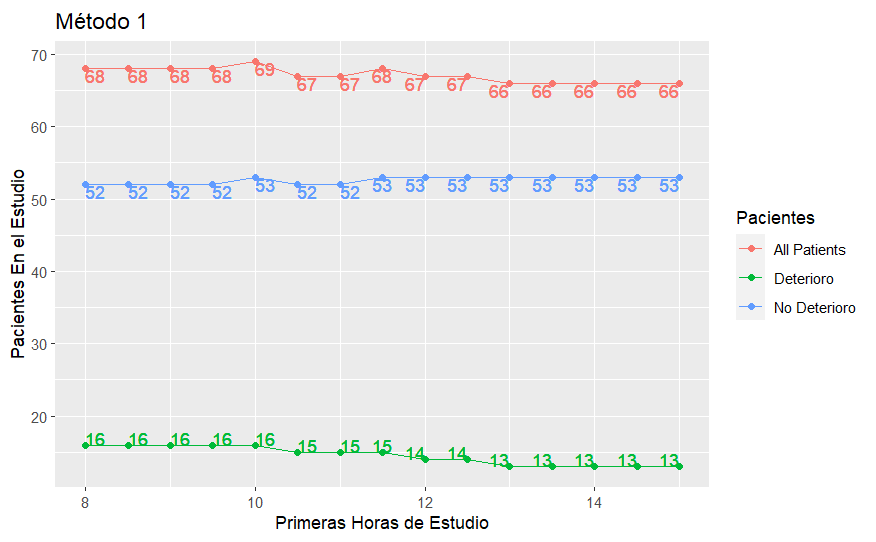
\includegraphics[scale = 1]{./img/metodo1.png}
    \caption{Método 1 de Exclusión de Pacientes}
    \label{fig:metodo1}
\end{figure}

\begin{figure}[H]
    \centering
    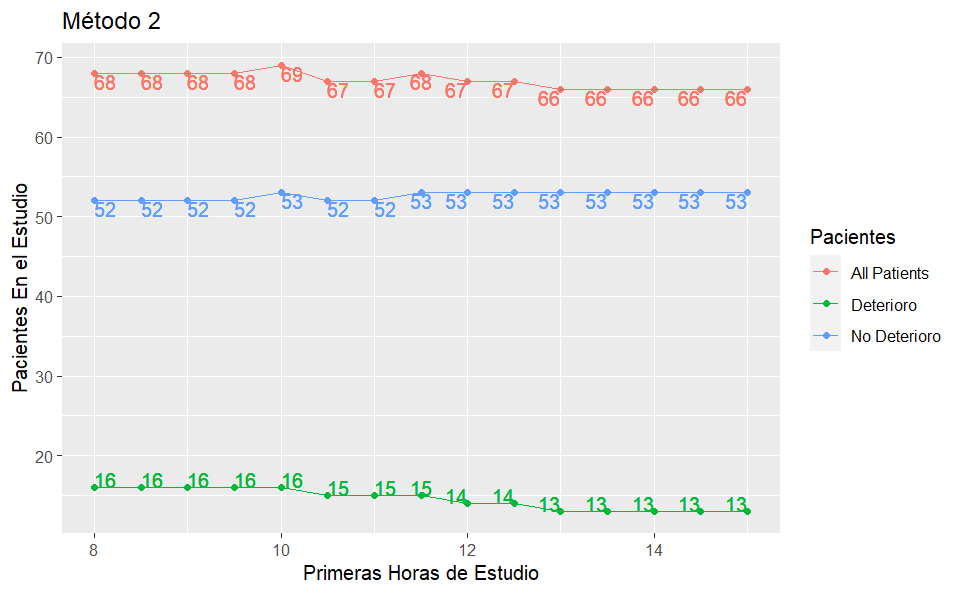
\includegraphics[scale = 1]{./img/metodo2.png}
    \caption{Método 2 de Exclusión de Pacientes}
    \label{fig:metodo2}
\end{figure}

Con los anteriores métodos se ha podido observar como realmente el hecho de ser más restrictivos con los datos faltantes no implica que se vayan a excluir muchas más pacientes y el cambio del ratio $ \text{Pacientes con Deterioro} / \text{PAcientes No Deterioro}$ es casi inapreciable. 

En la situación más restrictiva del \textit{Método 1} de la Figura \ref{fig:metodo1} el ratio es de $ \frac{16}{52} \approx 0.31 $ y en la situación menos restrictiva el ratio es de $ \frac{13}{53} \approx 0.245$. La variación total de pacientes a incluir en el estudio es de apenas un $3 \%$, se pasa de $68$ pacientes a excluir a $2$, obteniendo un total de $66$ pacientes. Cabe aclarar que la situación más restrictiva es aquella que considera más horas de monitorización manteniendo el \textit{threshold} en el $5 \%$ de valores faltantes., es decir la combinación de valores más alejada en el eje $x$ de la Figura \ref{fig:metodo1}.

Por otro lado el \textit{Método 2} de la figura \ref{fig:metodo2} en la situación más restrictiva el ratio es de $ \frac{14}{54} \approx 0.26$ y en la menos restrictiva es de $ \frac{16}{59} \approx 0.272$. En este caso si que existe un considerable aumento de la muestra de pacientes, se pasa de $68$ pacientes a $75$ aumentando en casi un $10 \%$ la muestra total. 

Para no alterar los datos debido a una posterior imputación y debido a que la variación de los datos es algo importante en el estudio se optará por establecer el \textit{threshold} en el $5 \%$ de valores faltantes, haciendo referencia a la siguiente entrada bibliográfica: \cite{Scheffer2002}. Se ha decidido que se estudiarán las primeras 24 horas de monitorización para mantener la unidad \textit{día} en el estudio ya que reduciendo el \textit{scope} no se consigue nada significativo. De esta forma se obtiene una muestra de $68$ pacientes y un ratio de $ \frac{14}{54} \approx 0.26 $.


muestra un comportamiento bastante parecido al \textit{Método 1}. En la situación menos restrictiva el ratio es de $ \frac{13}{53} \approx 0.245$. La variación total de pacientes a incluir en el estudio es de apenas un $3 \%$, se pasa de $68$ pacientes a excluir a $2$, obteniendo un total de $66$ pacientes.

En la siguiente tabla se muestra la cantidad de pacientes en el estudio:

\begin{table}[H]
    \centering
    \begin{tabular}{|m{2cm}|m{2.25cm}|m{2cm}|m{2cm}|}
    \hline
        Pacientes Totales & No Deterioro & Deterioro & Ratio \\ \hline
        68 & 54 & 14 & 0.26 \\ \hline
    \end{tabular}
    \caption{Pacientes Totales, con Deterioro, sin Deterioro y Ratio entre Deterioro y No Deterioro seleccionados para el estudio}
        \label{tabla:ratio-deterioro-P1}
\end{table}

\subsubsection{Imputación de Datos}\label{sec:imputacion-de-datos}

Una vez decidido los pacientes que se van a incluir en el estudio se ha de realizar una imputación de datos. 

La imputación de datos se hará en dos documentos diferentes:
\begin{itemize}
    \item \textbf{Archivo de Datos de Pacientes:} En este archivo se imputarán los datos faltantes de las variables \textit{Cuantitativas} y \textit{Cualitativas} de la Tabla \ref{tabla:cuali_cuanti}.
    \item \textbf{Carpeta de Datos de Monitorización:} En esta carpeta se imputarán los datos numéricos faltantes de las variables \textit{Series Temporales} de la Tabla \ref{tabla:variables_estudio}.
\end{itemize}

Cada imputación se hará de una manera diferente. En el primer caso ya que es necesario imputar datos de variables cualitativas y cuantitativas se utilizará el método de \textit{Distancia de Gower} y en el segundo caso se utilizará el método de \textit{k-Nearest Neighbor Imputation}. 

\paragraph*{Distancia de Gower}

La distancia de Gower puede utilizarse para medir la diferencia entre dos registros, que pueden contener una combinación de datos lógicos, numéricos, categóricos o textuales. La distancia es siempre un número comprendido entre 0 (idéntico) y 1 (máxima diferencia). La distancia de Gower se calcula como el promedio de las disimilitudes parciales entre individuos.

El coeficiente de disimilitud como lo define Gower en su artículo puede ser utilizado para medir la distancia entre dos puntos en un espacio multidimensional y puede ser calculado utilizando diferentes métodos; dependiendo del tipo de datos y del espacio en el que se encuentran los puntos. \cite{Gower1971}













